\section*{Analiza porównawcza spójności wyjaśnień}

W tej sekcji przeprowadzono ocenę spójności wyjaśnień generowanych przez różne metody XAI: LIME, SHAP i GradCAM.
Celem analizy było zrozumienie, jak bardzo wyjaśnienia nakładają się na siebie oraz jak różne techniki identyfikują istotne cechy obrazu.

W pierwszym etapie oceny spójności wyjaśnień każda z metod XAI została użyta do wygenerowania wyjaśnień dla tego samego zestawu obrazów.
Następnie wyniki zostały przedstawione za pomocą metryki IoU (Intersection over Union), która mierzy stopień pokrycia się regionów uznawanych za istotne przez różne metody.

\begin{figure}
	\centering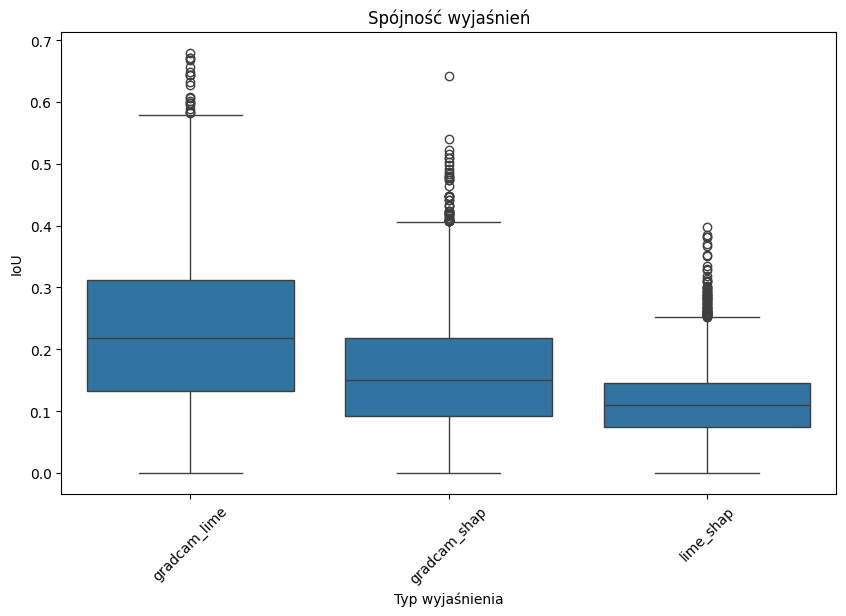
\includegraphics[width=.6\textwidth]{img/base_coherence}
	\caption{Spójność wyjaśnień}  \label{rys:base_coherence}
\end{figure}

Na wykresie pudełkowym (Rys \ref{rys:base_coherence}) przedstawione są wartości IoU dla porównania spójności wyjaśnień między różnymi metodami.

\begin{table}
	\centering
	\begin{tabular}{|c|c|}
		\hline
		\textbf{Metoda XAI} & \textbf{Średnie IoU} \\
		\hline
		GradCAM vs. LIME    & 0.210750             \\
		\hline
		GradCAM vs. SHAP    & 0.279382             \\
		\hline
		LIME vs. SHAP       & 0.113670             \\
		\hline
	\end{tabular}
	\caption{Średnie wartości IoU dla porównania spójności wyjaśnień}
	\label{tab:base_coherence}
\end{table}

Tabela \ref{tab:base_coherence} przedstawia średnie wartości IoU dla porównania spójności wyjaśnień między różnymi metodami XAI.

Wyniki pokazały, że największą spójność wykazały wyjaśnienia wygenerowane przez metody GradCAM i SHAP.
Natomiast najmniejszą spójność wykazały wyjaśnienia wygenerowane przez LIME i SHAP, co może wskazywać na różnice w podejściu tych metod do identyfikacji luczowych cech.

Aby dokładniej przeanalizować spójność wyjaśnień, podzielono dane ze względu na kategorie bazy danych ImageNetS.
Analiza została przeprowadzona dla różnych kategorii obrazów.

\begin{figure}
	\centering
	\begin{subfigure}[b]{0.3\textwidth}
		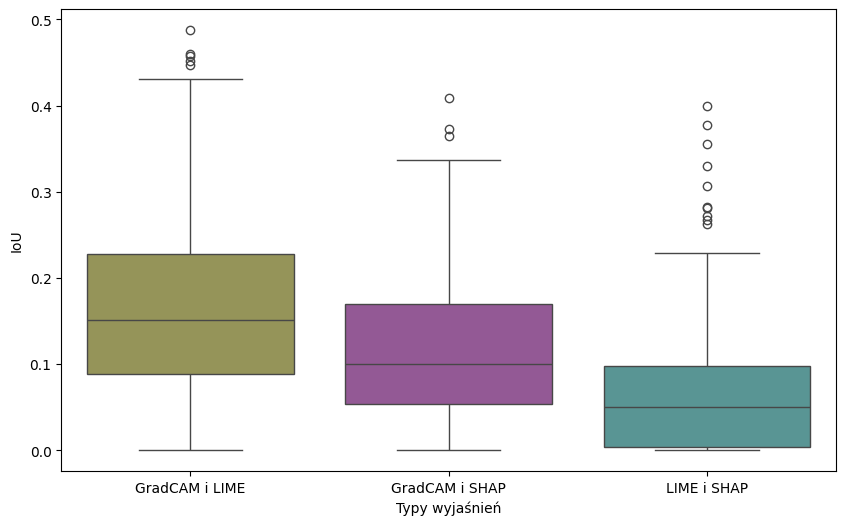
\includegraphics[width=.9\textwidth]{img/base_coherence_dog}
		\caption{Dog}  \label{}
	\end{subfigure}
	\begin{subfigure}[b]{0.3\textwidth}
		\centering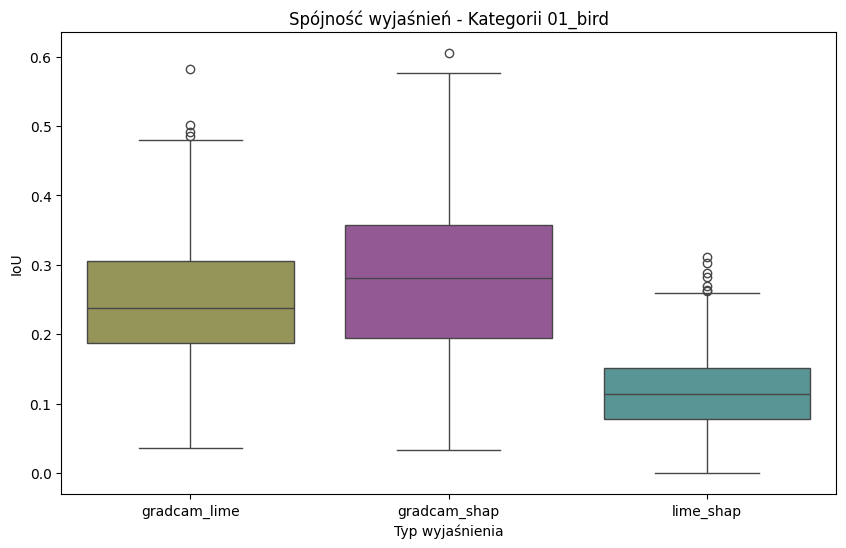
\includegraphics[width=.9\textwidth]{img/base_coherence_bird}
		\caption{Bird}  \label{}
	\end{subfigure}
	\begin{subfigure}[b]{0.3\textwidth}
		\centering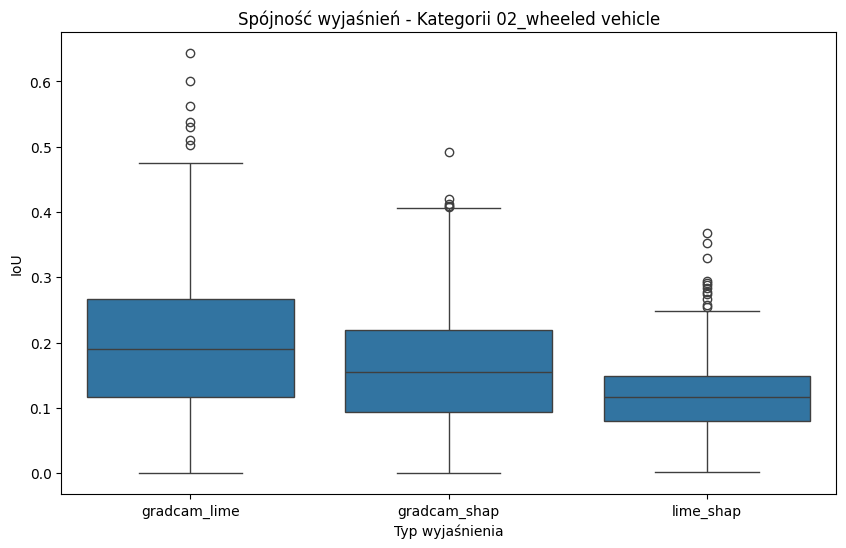
\includegraphics[width=.9\textwidth]{img/base_coherence_vehicle}
		\caption{Vehicle}  \label{}
	\end{subfigure}
	\begin{subfigure}[b]{0.3\textwidth}
		\centering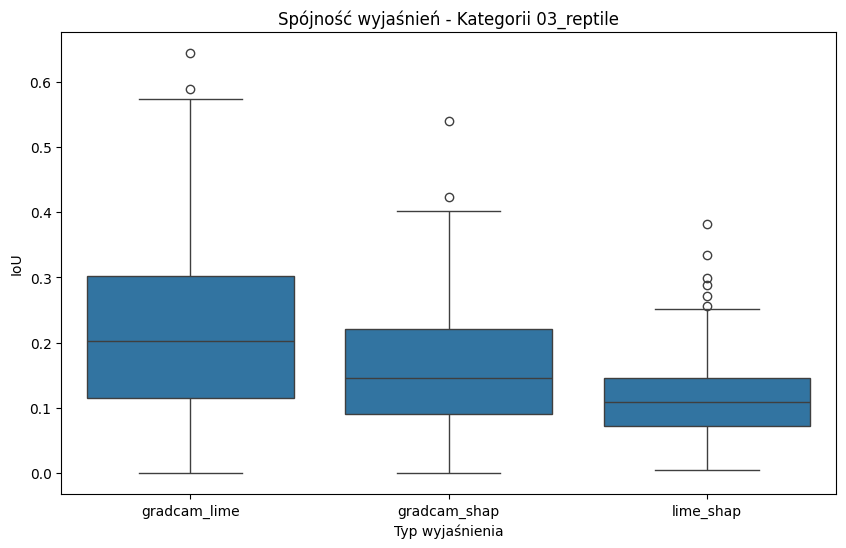
\includegraphics[width=.9\textwidth]{img/base_coherence_reptile}
		\caption{Reptile}  \label{}
	\end{subfigure}
	\begin{subfigure}[b]{0.3\textwidth}
		\centering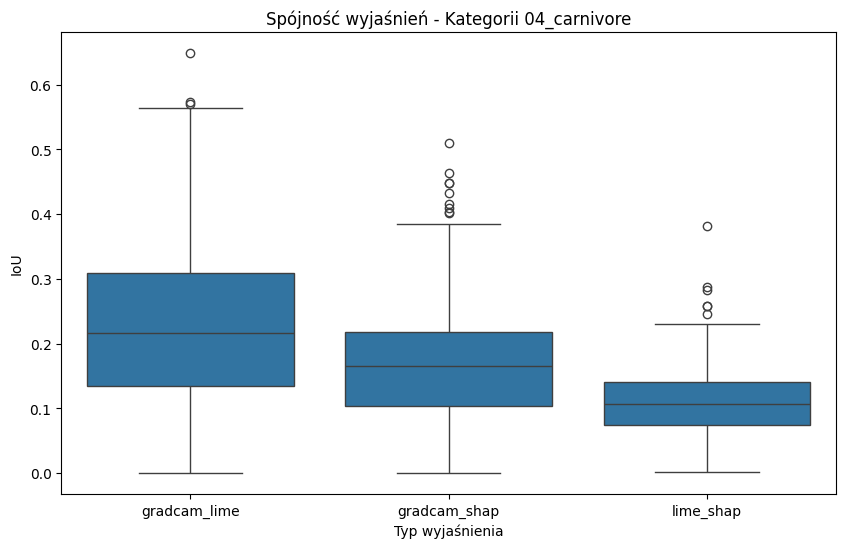
\includegraphics[width=.9\textwidth]{img/base_coherence_carnivore}
		\caption{Carnivore}  \label{}
	\end{subfigure}
	\begin{subfigure}[b]{0.3\textwidth}
		\centering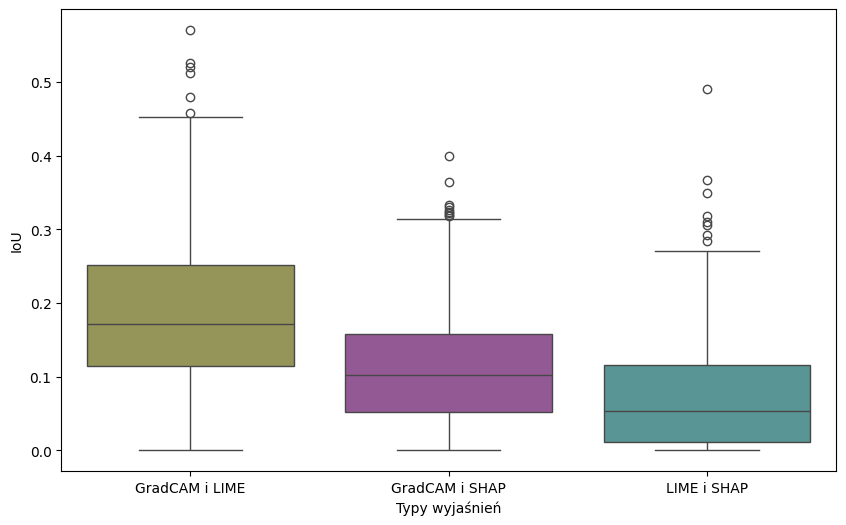
\includegraphics[width=.9\textwidth]{img/base_coherence_insect}
		\caption{Insect}  \label{}
	\end{subfigure}
	\begin{subfigure}[b]{0.3\textwidth}
		\centering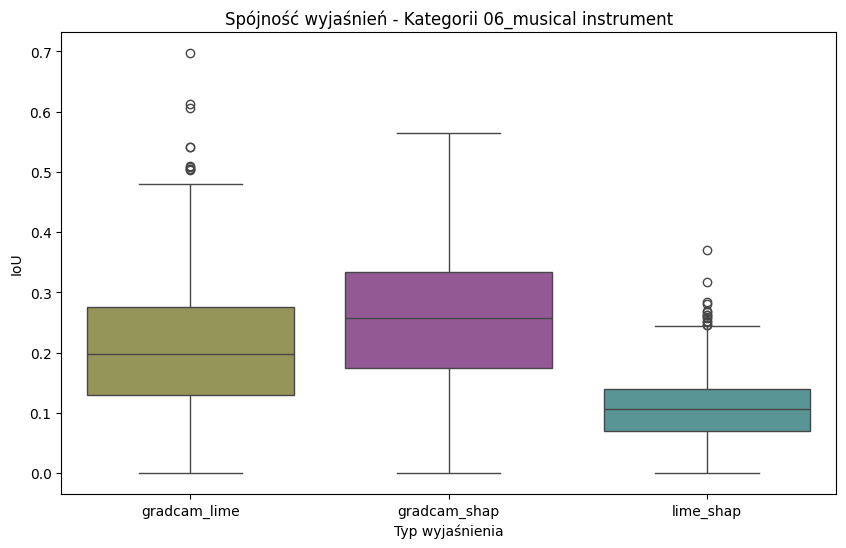
\includegraphics[width=.9\textwidth]{img/base_coherence_music}
		\caption{Instrument}  \label{}
	\end{subfigure}
	\begin{subfigure}[b]{0.3\textwidth}
		\centering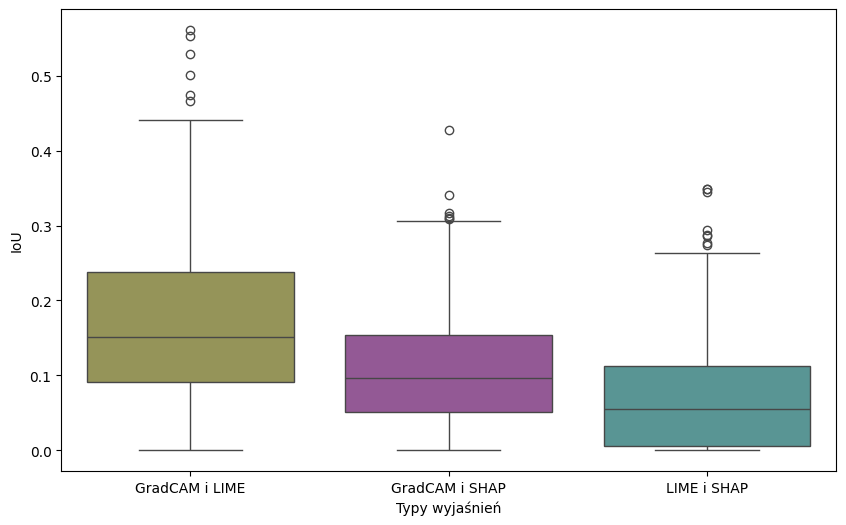
\includegraphics[width=.9\textwidth]{img/base_coherence_primate}
		\caption{Primate}  \label{}
	\end{subfigure}
	\begin{subfigure}[b]{0.3\textwidth}
		\centering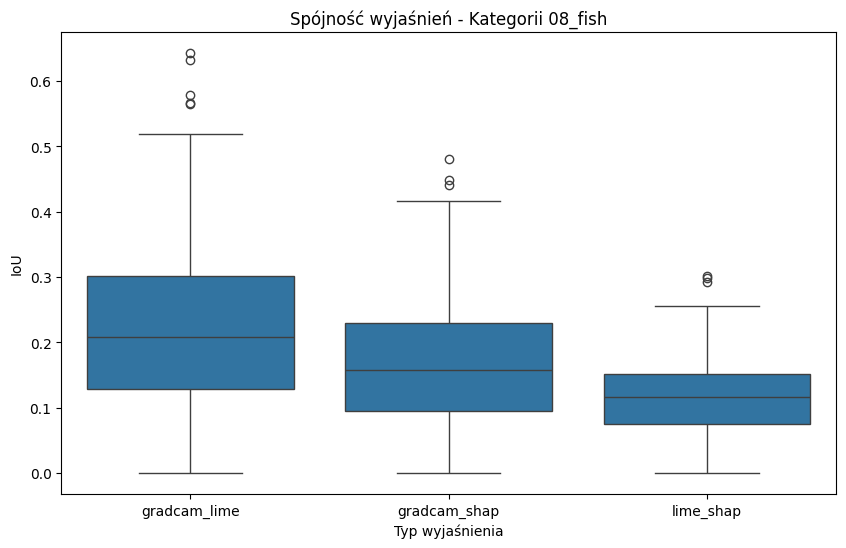
\includegraphics[width=.9\textwidth]{img/base_coherence_fish}
		\caption{Fish}  \label{}
	\end{subfigure}
	\caption{Spójność wyjaśnień dla różnych kategorii}
\end{figure}

\begin{table}[h]
	\centering
	\begin{tabular}{|c|c|c|c|}
		\hline
		\textbf{Kategoria}  & \textbf{GradCAM vs LIME} & \textbf{GradCAM vs SHAP} & \textbf{LIME vs SHAP} \\
		\hline
		Pies                & 0.206546                 & 0.277394                 & 0.111613              \\
		\hline
		Ptak                & 0.247909                 & 0.277716                 & 0.117751              \\
		\hline
		Pojazd na kołach    & 0.204956                 & 0.283621                 & 0.118001              \\
		\hline
		Gad                 & 0.191600                 & 0.287120                 & 0.113589              \\
		\hline
		Mięsorzerca         & 0.196739                 & 0.292880                 & 0.110058              \\
		\hline
		Insekt              & 0.235127                 & 0.273465                 & 0.119031              \\
		\hline
		Instrument muzyczny & 0.208132                 & 0.253540                 & 0.109638              \\
		\hline
		Naczelny            & 0.195163                 & 0.283483                 & 0.105888              \\
		\hline
		Ryba                & 0.210879                 & 0.285220                 & 0.117462              \\
		\hline
	\end{tabular}
	\caption{Średnie wartości IoU dla różnych kategorii}
	\label{tab:base_coherence_categories}
\end{table}

Tabela \ref{tab:base_coherence_categories} przedstawia średnie wartości IoU dla porównania spójności wyjaśnień w różnych kategoriach obrazów.

Różnice wartości IoU między kategoriami są relatywnie podobne, co wskazuje na konsystencję w wynikach pomiędzy różnymi typami obrazów.
Zawsze najwyższe wartości IoU odnotowano dla porównania GradCAM i SHAP, następnie GradCAM i LIME, a najniższe dla LIME i SHAP.

Niska spójność między LIME i SHAP, pomimo wyższej spójności GradCAM i LIME oraz GradCAM i SHAP, może wskazywać na to, że obszary identyfikowane przez GradCAM są większe i bardziej ogólne.

GradCAM działa na poziomie cech wysokiego poziomu, które są identyfikowane na końcowych warstwach sieci neuronowej.
W związku z tym, GradCAM ma tendencję do zaznaczania większych regionów na obrazie, które zawierają kluczowe cechy wpływające na klasyfikację.
Dzięki temu wyjaśnienia generowane przez GradCAM są bardziej ogólne i obejmują szersze obszary obrazu.

LIME i SHAP z kolei, działają na bardziej szczegółowych poziomach.

W rezultacie, większe i bardziej ogólne regiony identyfikowane przez GradCAM mają większe szanse na nakładanie się z wyjaśnieniami LIME oraz SHAP.
Natomiast LIME i SHAP, ze względu na swoją szczegółowość, wykazują mniejszą spójność, ponieważ identyfikują bardziej precyzyjne i różniące się od siebie obszary.

Aby zweryfikować czy wielkość wyjaśnień miała znaczenie przeanalizowano spójność wyjaśnień podzieloną ze względu na wielkość obiektów na obrazie.

\begin{figure}
	\centering
	\begin{subfigure}[b]{0.3\textwidth}
		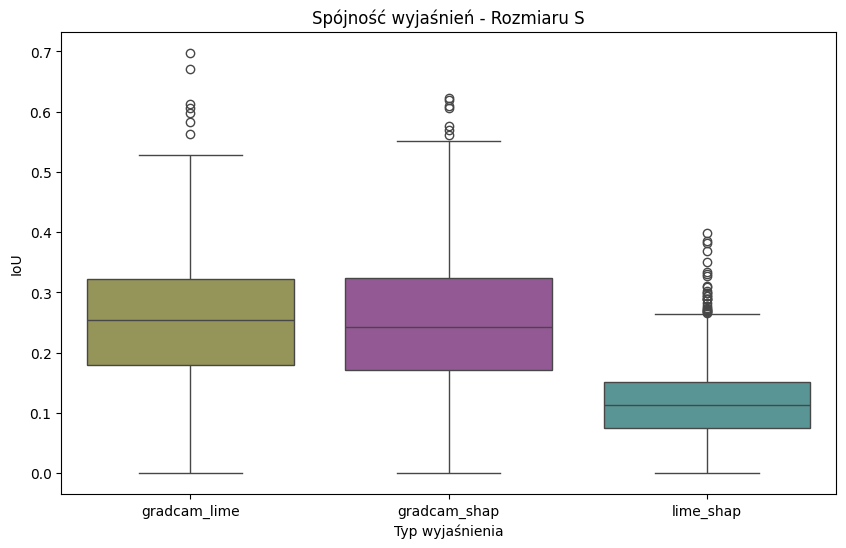
\includegraphics[width=.9\textwidth]{img/base_coherence_size_S}
		\caption{Mały}  \label{}
	\end{subfigure}
	\begin{subfigure}[b]{0.3\textwidth}
		\centering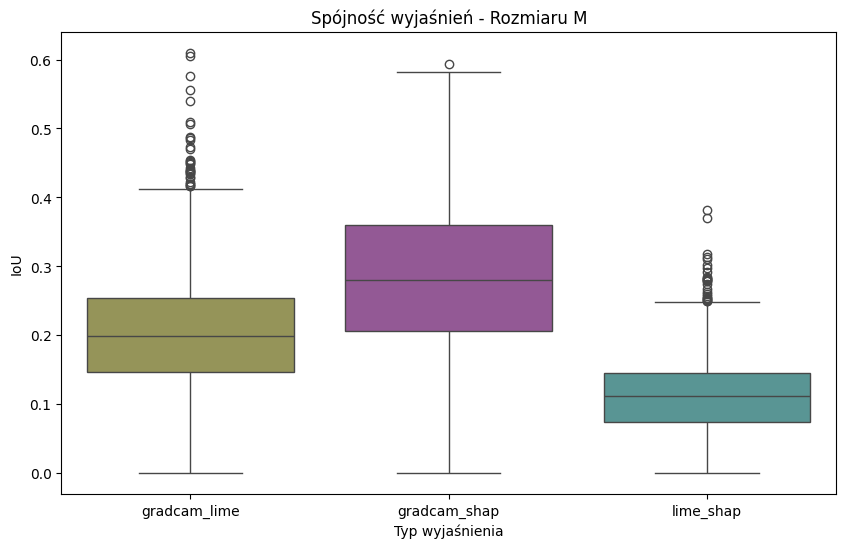
\includegraphics[width=.9\textwidth]{img/base_coherence_size_M}
		\caption{Średni}  \label{}
	\end{subfigure}
	\begin{subfigure}[b]{0.3\textwidth}
		\centering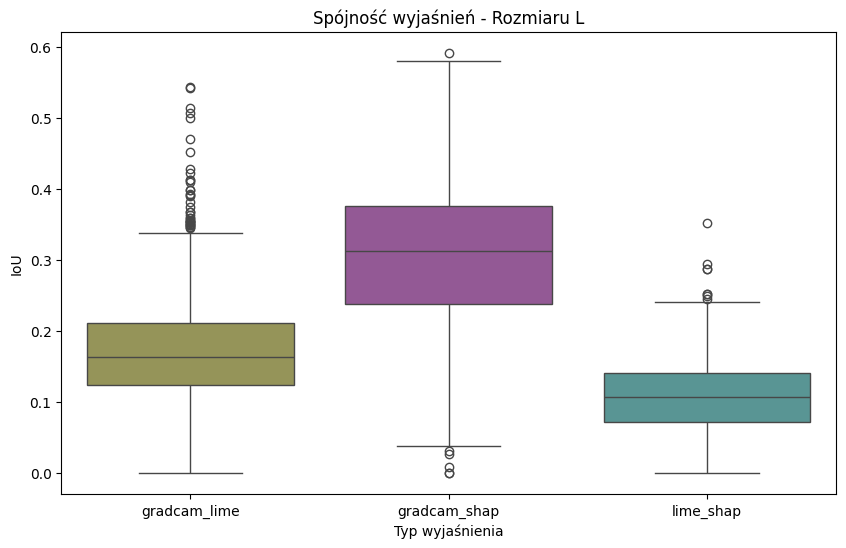
\includegraphics[width=.9\textwidth]{img/base_coherence_size_L}
		\caption{Duży}  \label{}
	\end{subfigure}
	\caption{Spójność wyjaśnień dla różnych rozmiarów}
\end{figure}

\begin{table}[h]
	\centering
	\begin{tabular}{|c|c|c|c|}
		\hline
		\textbf{Rozmiar} & \textbf{GradCAM vs LIME} & \textbf{GradCAM vs SHAP} & \textbf{LIME vs SHAP} \\
		\hline
		S                & 0.253597                 & 0.250014                 & 0.117247              \\
		\hline
		M                & 0.204279                 & 0.282094                 & 0.114313              \\
		\hline
		L                & 0.172506                 & 0.307551                 & 0.109135              \\
		\hline
	\end{tabular}
	\caption{Średnie wartości IoU dla różnych rozmiarów}
	\label{tab:base_coherence_size}
\end{table}

Tabela \ref{tab:base_coherence_size} przedstawia średnie wartości IoU dla porównania spójności wyjaśnień w zależności od rozmiaru obiektu na obrazie.

Wyniki:
\begin{itemize}
	\item \textbf{Rozmiar S} - Największa spójność wyjaśnień występuje między metodami GradCAM i LIME oraz GradCAM i SHAP.
	      Spójność między LIME i SHAP jest znacznie niższa tak jak w poprzednich analizach.
	\item \textbf{Rozmiar M} - GradCAM i SHAP ponownie wykazują największą spójność, następnie GradCAM i LIME, a najniższą spójność odnotowano między LIME i SHAP.
	\item \textbf{Rozmiar L} - Spójność wyjaśnień między GradCAM i SHAP jest najwyższa. GradCAM i LIME mają niższą spójność, a najniższą spójność obserwuje się między LIME i SHAP.
\end{itemize}

Dodatkowo zauważono, że spójność między GradCAM i LIME była odwrotnie proporcjonalna do wielkości obeiktu.
Im mnijeszy obiekt, tym większa była spójność między tymi metodami.
Podobny trend zaobserwowano w przypadku spójności między LIME i SHAP, choć wpływ wielkości obiektu był mniejszy.
Natomiast spójność między GradCAM i SHAP była proporcjonalnie zależna od wielkośći.
Im większy obiekt, tym większa była spójność między tymi metodami.

Warto zauważyć, że metody takie jak LIME i SHAP są wrażliwe na dobór parametrów.
Te zależności od parametrów mogą wpływać na stabilność i spójność wyjaśnień generowanych przez te techniki.
Co może częściowo tłumaczyć podobne wyniki między LIME i SHAP niezależnie od rozmiaru obiektu.

